\documentclass[a4paper,12pt]{article} % тип документа

% Поля страниц
\usepackage[left=2.5cm,right=2.5cm,top=2cm,bottom=2cm,bindingoffset=0cm]{geometry}
    
% Отступ после заголовка
\usepackage{indentfirst}

% Картинки
\usepackage{graphicx}
\graphicspath{{images/}}

% Таблицы
\usepackage{booktabs}
\usepackage{floatrow}

% Русский язык
\usepackage{cmap}  % поиск в PDF
\usepackage{mathtext}  % русские буквы в формулах
\usepackage[T2A]{fontenc}  % кодировка
\usepackage[utf8]{inputenc}  % кодировка исходного текста
\usepackage[english,russian]{babel}  % локализация и переносы

% Математика
\usepackage{amsmath}

% Ссылки TODO
% \usepackage[unicode=true]{hyperref}
% \usepackage[T1]{fontenc}

\begin{document}

\begin{center}   
	\large{Лабораторная работа № 1.3.3\\\textbf{Измерение вязкости воздуха по течению в тонких трубках}}\\
\end{center}

\section{Аннотация}

\noindent\textbf{Цель работы:}
экспериментально исследовать свойства течения газов по тонким трубкам при различных числах Рейнольдса; выявить область применимости закона Пуазейля и с его помощью определить коэффициент вязкости воздуха.\hfill
	
\bigskip
\noindent\textbf{В работе используются:}
система подачи воздуха (компрессор, поводящие трубки); газовый счетчик барабанного типа; спиртовой микроманометр с регулируемым наклоном; набор трубок различного диаметра с выходами для подсоединения микроманометра; секундомер.

\section{Теоретические сведения}

Согласно закону вязкости Ньютона:
$$\tau_{xy} = \eta \frac{\partial \upsilon_x}{\partial y},$$
где $\eta$ - коэффициент динамической вязкости.

Характер течения может быть ламинарным или турбулентным, определяется числом Рейнольдса:
\begin{equation}
Re = \frac{\rho u a}{\eta},
\end{equation} 
где $\rho$ - плотность среды, $u$ - характерная скорость потока, $a$ - характерный размер системы.

Из опыта известно, что переход к турбулентному течению по трубкам круглого сечения наблюдается при $Re_{кр} \approx 10^3$. Здесь в качестве характерного размера выбран радиус трубы $R$, а в качестве характерной скорости $u$ выбрана
средняя скорость потока, определяемая через полный расход $Q$:
\begin{equation}
\bar{u} = \frac{Q}{\pi R^2}.
\end{equation}

Формула Пуазейля позволяет найти вязкость газа по зависимости расхода от перепада
давления в трубе и используется в качестве основной расчётной формулы в данной работе:
\begin{equation}
Q = \frac{\pi R^4\Delta P}{8\eta l},
\end{equation}

Длину установления ламинарного течения можно оценить по формуле:
\begin{equation}\label{длина}
l_{\text{уст}} \approx 0.2R\cdot Re
\end{equation}

\newpage

\section{Используемое оборудование}

\subsection*{Экспериментальная установка}

Схема экспериментальной установки изображена на рисунке. Поток воздуха
под давлением, немного превышающим атмосферное, поступает через газовый счётчик в тонкие металлические трубки. Воздух нагнетается компрессором, интенсивность его подачи регулируется краном К. Трубки снабжены
съёмными заглушками на концах и рядом миллиметровых отверстий, к которым можно подключать микроманометр. В рабочем состоянии открыта заглушка на одной (рабочей) трубке, микроманометр подключён к двум её выводам, а все остальные отверстия плотно закрыты пробками.

Перед входом в газовый счётчик установлен водяной U-образный манометр. Он служит для измерения давления газа на входе, а также предохраняет
счётчик от выхода из строя. При превышении максимального избыточного
давления на входе счётчика ($\approx$ 30 см вод. ст.) вода выплёскивается из трубки
в защитный баллон Б, создавая шум и привлекая к себе внимание экспериментатора.

\begin{figure}[h!]
    \centering
    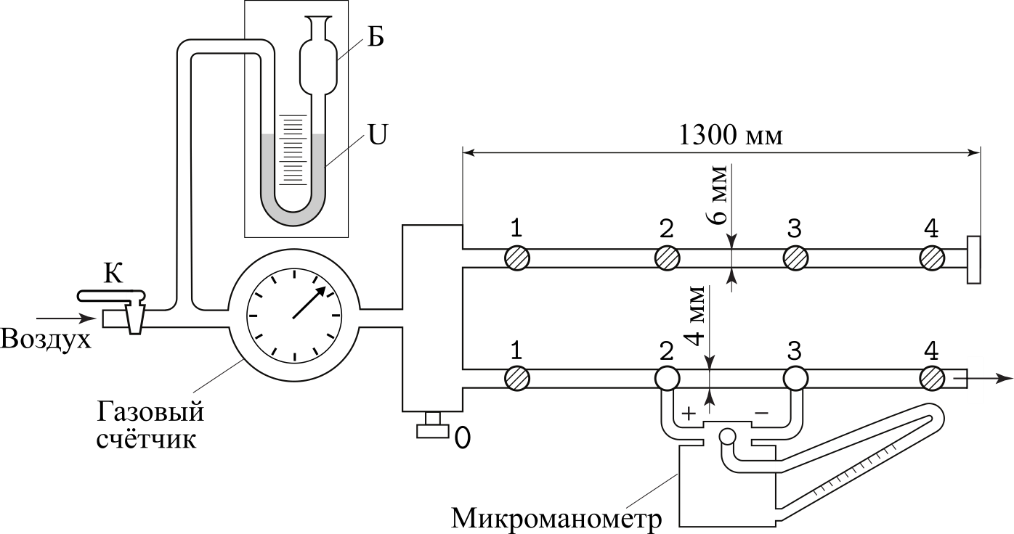
\includegraphics[width=\textwidth]{установка.png}
    \caption{Экспериментальная установка}
\end{figure}

\subsection*{Газовый счётчик}

В работе используется газовый счётчик барабанного
типа, позволяющий измерять объём газа $\Delta V$, прошедшего через систему. Измеряя время $\Delta t$ при помощи секундомера, можно вычислить средний объёмный расход газа $Q = \Delta V / \Delta t$ (для получения массового расхода [кг/с] результат
необходимо домножить на плотность газа $\rho$).
Работа счётчика основана на принципе вытеснения: на цилиндрической ёмкости жёстко
укреплены лёгкие чаши (см. рис. \ref{газосчетчик}, где для
упрощения изображены только две чаши), в которые поочередно поступает воздух из входной
трубки расходомера. Когда чаша наполняется,
она всплывает и её место занимает следующая
и т.д. Вращение оси предаётся на счётно-суммирующее устройство.
Для корректной работы счётчика он должен
быть заполнен водой и установлен горизонтально по уровню (подробнее см. техническое
описание установки).

\begin{figure}[h!]
    \centering
    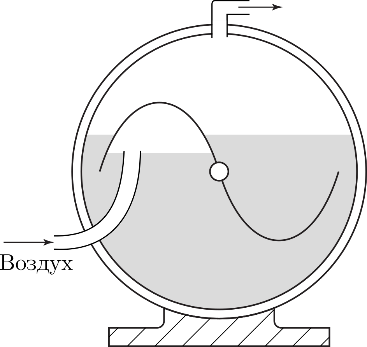
\includegraphics[width=0.4\textwidth]{газосчетчик.png}
    \caption{Принцип работы барабанного газосчётчика}\label{газосчетчик}
\end{figure}

\newpage

\subsection*{Микроманометр}

В работе используется жидкостный манометр с наклонной трубкой. Разность давлений на входах манометра измеряется по высоте
подъёма рабочей жидкости (как правило, этиловый спирт). Регулировка
наклона позволяет измерять давление в различных диапазонах.

На крышке прибора установлен трехходовой кран, имеющий два рабочих
положения — (0) и (+). В положении (0) производится установка мениска жидкости на ноль, что необходимо сделать перед началом работы (в процессе работы также рекомендуется периодически проверять положение нуля). В положении (+) производятся измерения.

При работе с жидкостным манометром важно не допустить его «зашкаливания» — перелива рабочей жидкости в подводящие трубки (в этом случае
работу придется приостановить для просушки трубок, долива спирта и т.д.).
Все манипуляции по перестановке измерительных трубок следует проводить,
когда манометр находится в положении (0). Подачу газа в систему, наоборот,
следует осуществлять в положении (+), чтобы контролировать величину давления и иметь возможность вовремя перекрыть поток.

Перед началом работы с микроманометром необходимо убедиться, что в
нём залито достаточное количество спирта, а сам манометр установлен строго
горизонтально по уровням. Подводящие трубки, заполненные спиртом, не
должны содержать пузырьков воздуха, а в трубках, заполненных воздухом, не
должно быть капель спирта. Подробнее инструкцию по подготовке прибора к
работе см. в техническом описании установки.

\newpage

\section{Результаты измерений}

\subsection*{Параметры окружающей среды}

$T=(299.25 \pm 0.10)$ К

$P=(97610 \pm 10)$ Па

\subsection*{Ламинарное и турбулентное течение}

\begin{table}[ht!]
\caption{$d=(3.95 \pm 0.05)$ мм, $l=(50.0 \pm 1.0)$ см}
\begin{tabular}{ cc }
\begin{tabular}{c|c|c|c}
\toprule
$\Delta t$, c & $N$ & $Q$, мл/с & $\Delta P$, Па \\
\midrule
12.80 & 63 & 78.12 & 122.45 \\
17.30 & 47 & 57.80 & 91.35 \\
19.90 & 40 & 50.25 & 77.75 \\
24.20 & 34 & 41.32 & 66.09 \\
26.60 & 30 & 37.59 & 58.31 \\
33.70 & 24 & 29.67 & 46.65 \\
41.70 & 20 & 23.98 & 38.87 \\
52.80 & 15 & 18.94 & 29.16 \\
84.20 & 10 & 11.88 & 19.44 \\
\bottomrule
\end{tabular}

\begin{tabular}{rrrr}
\toprule
$\Delta t$, $c$ & $N$ & $\Delta P$, $Па$ & $Q$, $мл/с$ \\
\midrule
9.6 & 101 & 196.3 & 104.2 \\
9.1 & 120 & 233.2 & 109.9 \\
8.5 & 154 & 299.3 & 117.6 \\
8.0 & 171 & 332.4 & 125.0 \\
7.8 & 186 & 361.5 & 128.2 \\
7.4 & 206 & 400.4 & 135.1 \\
6.7 & 247 & 480.1 & 149.3 \\
6.2 & 277 & 538.4 & 161.3 \\
\bottomrule
\end{tabular}

\end{tabular}
\end{table}

\begin{table}[ht!]
\caption{$d=(3.95 \pm 0.05)$ мм, $l=(90.0 \pm 1.0)$ см}
\begin{tabular}{ cc }
\begin{tabular}{c|c|c|c}
\toprule
$\Delta t$, c & $N$ & $Q$, мл/с & $\Delta P$, Па \\
\midrule
16.60 & 93 & 60.24 & 180.76 \\
19.20 & 80 & 52.08 & 155.50 \\
22.00 & 70 & 45.45 & 136.06 \\
25.30 & 60 & 39.53 & 116.62 \\
30.80 & 50 & 32.47 & 97.18 \\
42.90 & 35 & 23.31 & 68.03 \\
78.60 & 20 & 12.72 & 38.87 \\
\bottomrule
\end{tabular}

\begin{tabular}{c|c|c|c}
\toprule
$\Delta t$, c & $N$ & $Q$, мл/с & $\Delta P$, Па \\
\midrule
12.10 & 130 & 82.64 & 252.68 \\
11.10 & 143 & 90.09 & 277.95 \\
10.50 & 155 & 95.24 & 301.27 \\
10.20 & 165 & 98.04 & 320.71 \\
9.90 & 176 & 101.01 & 342.09 \\
9.70 & 185 & 103.09 & 359.58 \\
9.40 & 212 & 106.38 & 412.06 \\
\bottomrule
\end{tabular}

\end{tabular}
\end{table}

\begin{table}[ht!]
\caption{$d=(5.30 \pm 0.05)$ мм, $l=(40.0 \pm 1.0)$ см}
\begin{tabular}{ cc }
\begin{tabular}{rrrr}
\toprule
$\Delta t$, $c$ & $N$ & $\Delta P$, $Па$ & $Q$, $мл/с$ \\
\midrule
7.0 & 35 & 68.0 & 142.9 \\
7.5 & 30 & 58.3 & 133.3 \\
8.8 & 25 & 48.6 & 113.0 \\
10.9 & 20 & 38.9 & 91.7 \\
13.9 & 15 & 29.2 & 71.9 \\
\bottomrule
\end{tabular}

\begin{tabular}{rrrr}
\toprule
$\Delta t$, $c$ & $N$ & $\Delta P$, $Па$ & $Q$, $мл/с$ \\
\midrule
6.3 & 53 & 103.0 & 158.7 \\
5.4 & 75 & 145.8 & 185.2 \\
4.6 & 102 & 198.3 & 217.4 \\
3.8 & 142 & 276.0 & 263.2 \\
3.6 & 166 & 322.7 & 277.8 \\
\bottomrule
\end{tabular}

\end{tabular}
\end{table}

\newpage

\section{Обработка данных}

\subsection*{Графики}

\begin{figure}[h!]
\begin{center}
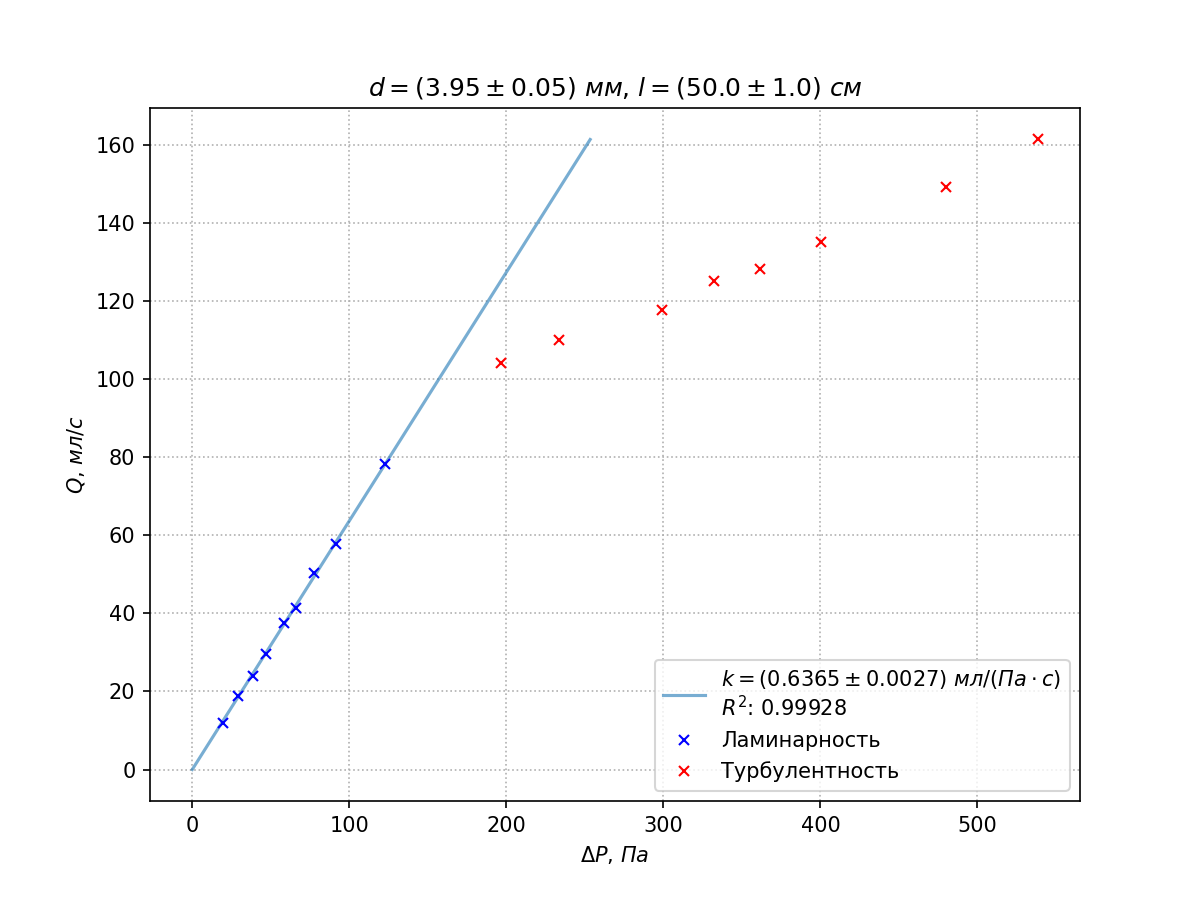
\includegraphics[width=0.89\textwidth]{Q(P)1.png}
\end{center}
\end{figure}

\begin{figure}[h!]
\begin{center}
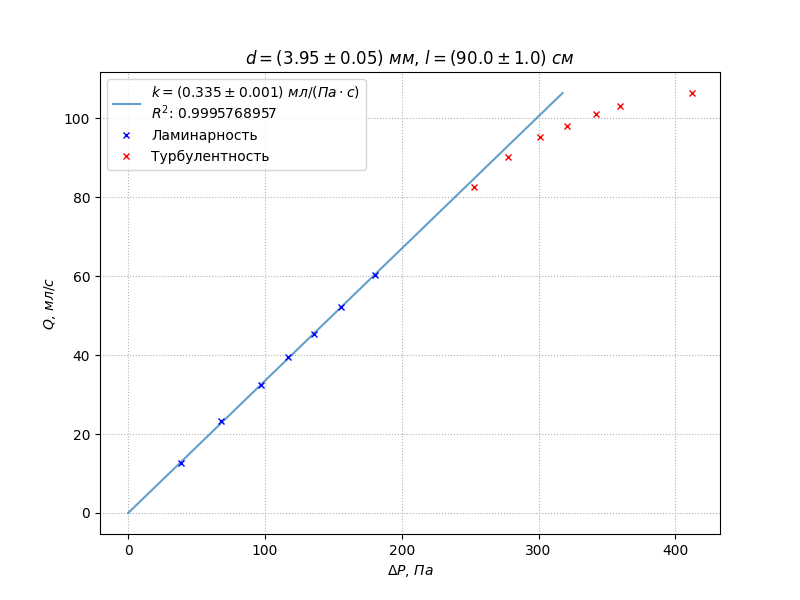
\includegraphics[width=0.89\textwidth]{Q(P)2.png}
\end{center}
\end{figure}

\begin{figure}[h!]
\begin{center}
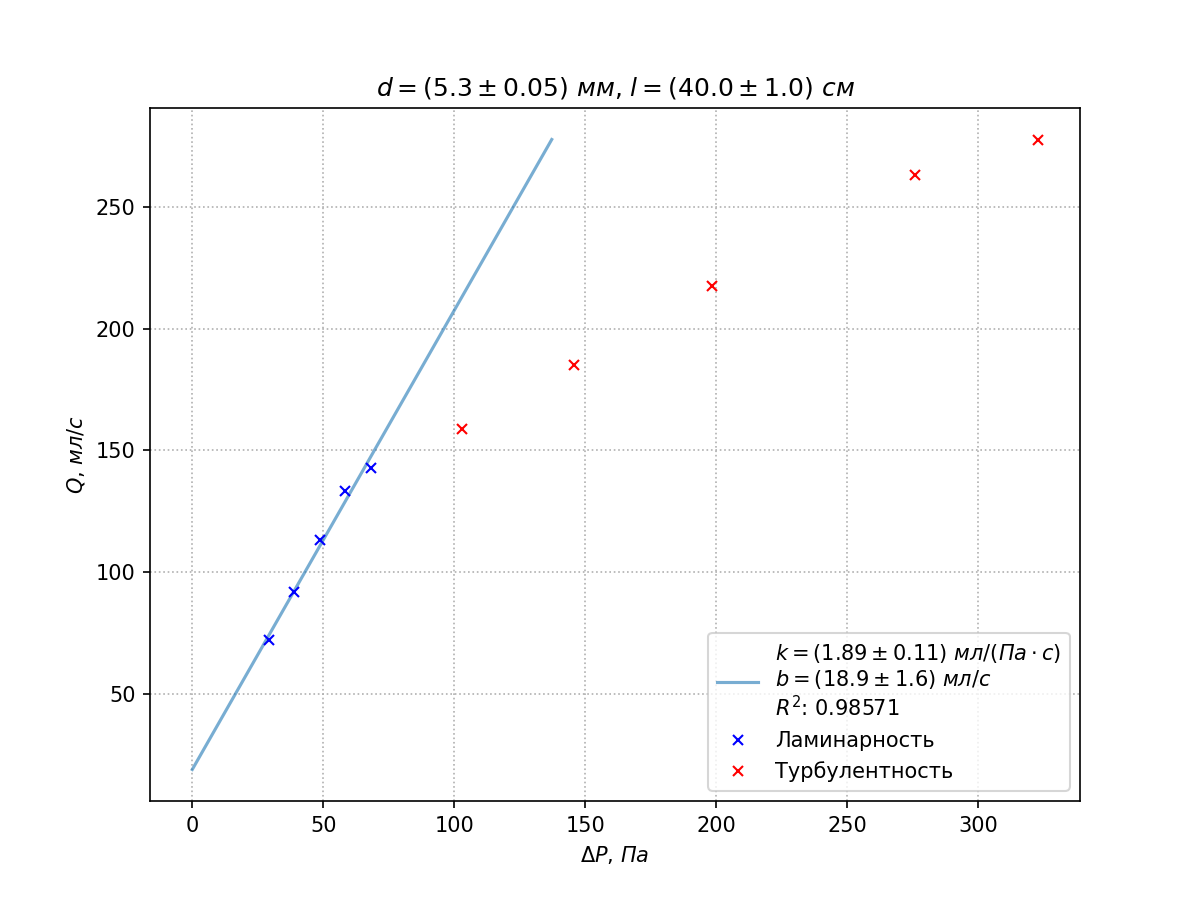
\includegraphics[width=0.89\textwidth]{Q(P)3.png}
\end{center}
\end{figure}

\subsection*{Обработка данных}

\begin{tabular}{rrr}
\toprule
$T$, $^\circ C$ & $\sigma$, $мН/м$ & $\sigma_{\sigma}$, $мН/м$ \\
\midrule
25.1 & 63.4 & 1.1 \\
30.3 & 62.6 & 1.1 \\
35.2 & 61.7 & 1.1 \\
40.2 & 60.8 & 1.1 \\
45.2 & 60.3 & 1.1 \\
50.2 & 59.7 & 1.1 \\
55.2 & 58.7 & 1.1 \\
60.1 & 57.6 & 1.0 \\
\bottomrule
\end{tabular}


\subsection{Обсуждение результатов}

Для каждой трубки по графику определена граница перехода от ламинарного участка к турбулентному. Для первых двух участков реузльтаты сошлись с теоретическими и теми, что были определны визуально в процессе снятия измерений. Для последнего участка выявлено отклонение, причной которого может быть большой диаметр трубки.

Зависимость $Q(\Delta P)$ на ламинарном участке соответствует линейной. Исключением являются последние две точки на последнем участке.

Пользуясь формулой Пуазейля, по угловым коэффициентам линейных участков определена взякость воздуха, которая в пределах погрешности сходится с табличными знаениями для всех участков.

Рассчитано критическое число Рейнольдса, которое по порядку сошлось с предполагаемым значением для все участков.

\end{document}